\sectioncounter{44}

\section{抛物线及其方程}

\subsection{知识梳理}
设定直线 $l$ 和定点 $F$ 满足 $F\notin l$. 若点 $P$ 到 $F$ 的距离等于 $P$ 到 $l$ 的距离, 则称点 $P$ 的轨迹为抛物线, 记为 $C$, 点 $F$ 和直线 $l$ 分别为抛物线 $C$ 的焦点和准线, $F$ 到 $l$ 的距离称为焦准距.

过点 $F$ 作 $l$ 的垂线 $FA$, 则 $|FA|$ 为焦准距, 设为 $p$. 以 $AF$ 所在直线为 $x$ 轴, 线段 $AF$ 的中垂线为 $y$ 轴, 建立如图 \ref{fig-190325-2010} 所示的平面直角坐标系, 则 $F\Big(\dfrac{p}2,0\Big)$, $l\colon x=-\dfrac{p}2$.

\begin{figure}[htb]
    \centering
    \begin{tikzpicture}[scale=0.5]
      \draw[\myaxisarrow] (-2,0) -- (4,0) 
        node[below] {$x$} coordinate(x axis);
      \draw[\myaxisarrow] (0,-3.5) -- (0,4) 
        node[left] {$y$} coordinate(y axis);
      \draw[line width=0.5pt,smooth,samples=100,domain=0:3] 
        plot(\x,{2*sqrt(\x)});
      \draw[line width=0.5pt,smooth,samples=100,domain=0:3] 
        plot(\x,-{2*sqrt(\x)});
      \draw [line width=0.5pt] (-1,-3.5)--(-1,3.8);
      \draw [line width=0.5pt] (1,0)--(2,2.8284);
      \draw [line width=0.5pt] (-1,2.8284)--(2,2.8284);
      
      \draw [fill=black] (1,0.) circle (1pt);
      \draw[color=black] (2,-1) node {$F\Big(\dfrac{p}2,0\Big)$};
      \draw [fill=black] (2,2.8284) circle (1pt);
      \draw[color=black] (2.4,2.4) node {$P$};
      \draw [fill=black] (-1,0) circle (1pt);
      \draw (-1,0.4) node[left] {$A$};
      \draw [fill=black] (-1,2.8284) circle (1pt);
      \draw (-1,2.8284) node[left] {$B$};
      \draw (-1,-2.5) node[left] {$l\colon x=-\dfrac{p}2$};
      \draw (-0.4,-0.5) node {$O$};
    \end{tikzpicture}
    \caption{}\label{fig-190325-2010}
\end{figure}

设 $P(x,y)$, 由抛物线的定义
\[\Big|x-\Bigl(-\frac{p}2\Bigr)\Big|
    = \sqrt{\Big(x-\frac{p}2\Big)^2+y^2},\]
平方整理得 $C\colon y^2=2px$ ($p>0$). 此方程为顶点在原点、对称轴为坐标轴的抛物线的四个标准方程之一,
\mymarginpar{注意四个标准方程对应图形的开口方向和所在象限.}
另外三个分别为 $y^2=-2px$, $x^2=2py$ 和 $x^2=-2py$ ($p>0$). 由抛物线的标准方程可知, 抛物线为轴对称图形, 对称轴与抛物线的交点称为顶点. 二次函数的图形也是抛物线, 可由抛物线 $x^2= 2py$ 平移得到.

抛物线的离心率 $e$ 定义为 $1$. 圆、椭圆、双曲线和抛物线统称为圆锥曲线, 它们都可以由某平面截圆锥面得到. 后三者可以利用焦点、准线和离心率给出统一的定义, 椭圆和双曲线的情形可以参考教材例题. 在求解与抛物线相关的问题时, 应充分利用抛物线的定义来简化计算, 有时还需借助图形的几何性质.

\lianxi
\begin{exercise}
    顶点在原点的抛物线 $C$ 的准线 $l\colon x=1$, 求该抛物线的焦准距和标准方程.
\end{exercise}
\beginsolution
    由题意, $C$ 的焦点为 $(-1,0)$, 焦准距 $p=2$, 标准方程为 $y^2= -4x$.
\endsolution

\begin{exercise}
    设抛物线 $C$ 的中心在原点, 焦点 $F$ 在坐标轴上, 且 $C$ 过点 $A(2,4)$, 求抛物线 $C$ 的标准方程.
\end{exercise}
\beginsolution
    困为点 $A(2,4)$ 在第一象限, 所以 $C$ 的标准方程只能为 $y^2= 2px$ 或 $x^2= 2py$ ($p>0$). 将 $A(2,4)$ 分别代入知, 所求方程为 $y^2= 8x$ 或 $x^2= y$.
\endsolution

\begin{exercise}
    设抛物线 $C$ 的顶点在原点, 对称轴为坐标轴, 焦点在直线 $l\colon 2x-y+4=0$ 上, 求该抛物线的标准方程.
\end{exercise}
\beginsolution
    $C$ 的焦点为 $l$ 与坐标轴的交点 $A(-2,0)$ 或 $B(0,4)$, 则 $C$ 的标准方程为 $y^2= -8x$ 或 $x^2= 16y$.
\endsolution

\begin{exercise}
    已知抛物线 $C\colon y^2= x$ 的焦点为 $F$, $C$ 上一点 $A(x_0,y_0)$ 满足 $|AF|= \dfrac54 x_0$, 求 $x_0$ 的值.
\end{exercise}
\beginsolution
    $C$ 的准线 $l\colon x= -\dfrac14$, 由抛物线的定义, 点 $A$ 到 $l$ 的距离等于 $|AF|$, 即
    \[x_0+ \frac14= \frac54 x_0,\quad x_0= 1.\]
\endsolution

\begin{exercise}
    若点 $P(x_0,4)$ 在抛物线 $C\colon y^2 =-8x$ 上, $F$ 是 $C$ 的焦点, 求 $|PF|$ 的值.
\end{exercise}
\beginsolution
    将点 $P(x_0,4)$ 代入 $C$ 的方程, 得 $x_0= -2$. 而抛物线 $C$ 的准线 $l\colon x=2$, 由抛物线的定义, $|PF|$ 等于点 $P$ 到 $l$ 的距离 $2-x_0$, 即 $|PF|= 4$.
\endsolution

\subsection{要点导学\quad 各个击破}
\subsubsection{求抛物线的方程}
\begin{example}
    已知点 $A$ 在抛物线 $C\colon y^2 =2px$ ($p>0$) 上, $F$ 为 $C$ 的焦点, $O$ 为原点, $|AF|= 4$ 且 $\angle OFA= 120^\circ$, 求抛物线 $C$ 的方程.
\end{example}
\beginsolution
    $F\Bigl(\dfrac{p}2,0\Bigr)$, 准线 $l\colon x= -\dfrac{p}2$. 设 $A(x_0,y_0)$, 由抛物线的定义和题意,
    \[|AF|= x_0+ \frac{p}2= 4.\]
    由 $\angle OFA= 120^\circ$ 作图知, $x_0= \dfrac{p}2+ 2$, 与上式联立解得, $p=2$. 所以 $C$ 的方程为 $y^2= 4x$.
\endsolution

\lianxi
\begin{exercise}[s]
    设抛物线 $C_1\colon y^2= 8px$ ($p>0$) 的焦点为 $F$, $C_1$ 与抛物线 $C_2\colon x^2= py$ 在第一象限的交点为 $M$, 且 $|MF|= 4$, 求抛物线 $C_2$ 的方程.
\end{exercise}
\beginsolution
    将 $C_1,C_2$ 的方程联立知, $M(2p,4p)$. 而 $C_1$ 的准线 $l_1\colon x= -2p$, 由抛物线的定义和题意,
    \[|MF|= 2p-(-2p)= 4,\quad p=1.\]
    所以 $C_2$ 的方程为 $x^2= y$.
\endsolution

\subsubsection{直线与抛物线的问题}
\begin{example}
    设抛物线 $C\colon y^2 =4x$ 的焦点为 $F$, 过点 $F$ 的直线交抛物线 $C$ 于 $A$,$B$ 两点, 点 $O$ 是坐标原点. 若 $|AF|= 5$, 求 $\triangle AOB$ 的面积.
\end{example}
\beginsolution
    $F(1,0)$, 准线 $l\colon x=-1$. 设 $A(x_A,y_A)$, 由抛物线的定义和题意,
    \[|AF|= x_A+1= 5,\quad x_A= 4,\]
    则 $y_A^2= 16$. 不妨设 $A(4,4)$, 则
    \[AF\colon y= \dfrac43(x-1),\]
    与 $C\colon y^2= 4x$ 联立解得, $x=4$, $\dfrac14$, 则 $B\Bigl(\dfrac14,-1\Bigr)$, 并记为 $(x_B,y_B)$. 所以 $\triangle AOB$ 的面积为
    \[S_{\triangle AOF}+ S_{\triangle BOF}
    = \frac12 |OF|(|y_A|+ |y_B|)= \frac{17}{8}.\]
\endsolution

\begin{example}
    已知抛物线 $C\colon y^2=4x$, 点 $O$ 是坐标原点, 过点 $M(-1,0)$ 的动直线 $l$ 与抛物线 $C$ 交于 $A$,$B$ 两点, 求证: $\overrightarrow{OA}\cdot\overrightarrow{OB}$ 为定值.
\end{example}
\beginsolution
    $l$ 的斜率显然存在, 设为 $k$, 则 $l\colon y= k(x+1)$, 与 $C\colon y^2=4x$ 联立,
    \[k^2x^2+ (2k^2-4)x+ k^2= 0.\]
    设 $A(x_1,y_1)$, $B(x_2,y_2)$, 则
    \[x_1+x_2= \frac{4-2k^2}4,\quad x_1x_2= 1.\]
    结合 $\overrightarrow{OA}\cdot\overrightarrow{OB}= x_1x_2+ y_1y_2$ 知, 
    \mymarginpar{此题可以一般化: 设定点 $M(m,0)$, 则
    \[\overrightarrow{OA}\cdot\overrightarrow{OB}= m^2-4m.\]}
    \[\begin{aligned}
        \overrightarrow{OA}\cdot\overrightarrow{OB}
        &= x_1x_2+ k^2(x_1+1)(x_2+1)\\
        &= (1+k^2)x_1x_2+ k^2(x_1+x_2)+ k^2\\
        &= 5.
    \end{aligned}\]
\endsolution

\lianxi
\begin{exercise}[s]
    抛物线 $C\colon y^2 =4x$ 的焦点为 $F$, 过点 $F$ 且倾斜角为 $60^\circ$ 的直线与 $C$ 分别交于 $A$,$B$ 两点, 点 $A$ 在第一象限, 求 $\dfrac{|AF|}{|BF|}$ 的值.
\end{exercise}
\beginsolution
    方法一: $F(1,0)$, $AB\colon y= \sqrt3(x-1)$ 与 $C\colon y^2 =4x$ 联立,
    \[3x^2- 10x+ 3= 0,\quad x=3,\frac13.\]
    设 $A(x_1,y_1)$, $B(x_2,y_2)$, 则 $x_1= 3$, $x_2= \dfrac13$. 由准线 $l\colon x=-1$ 和抛物线的定义,
    \[|AF|= x_1+1= 4,\quad |BF|= x_2+1= \frac43.\]
    所以 $\dfrac{|AF|}{|BF|}= 3$.

    方法二:准线 $l\colon x=-1$, 过点 $A$,$B$ 分别向 $l$ 作垂线, 垂足设为 $C$ 和 $D$. 由抛物线的定义可设
    \mymarginpar{方法一为代数法, 方法二为几何法, 都用了抛物线的定义. 方法二也可用于椭圆和双曲线的情形 (需借助另一种定义).}
    \[|AF|= |AC|= m,\quad |BF|= |BD|= n.\]
    再过点 $B$ 作 $BE\perp AC$ 于点 $E$, 则四边形 $CDBE$ 为矩形, 
    \[|AE|= |AC|- |BD|= m-n.\]
    由 $\angle BAE= 60^\circ$ 知, $|AB|= 2|AE|$, 即
    \[m+n= 2(m-n),\quad \frac{m}{n}= \frac13.\]
\endsolution

\subsubsection{课堂评价}
\begin{exercise}
    设抛物线 $C\colon y^2 =4x$ 的焦点为 $F$, 过点 $F$ 的直线交 $C$于 $A$,$B$ 两点, 若线段 $AB$ 中点的横坐标为 $3$, 求 $|AB|$ 的值.
\end{exercise}
\beginsolution
    准线 $l\colon x=-1$, 设 $A(x_1,y_1)$, $B(x_2,y_2)$, 则
    \mymarginpar{类似地, 若过焦点的直线与抛物线交于点 $A$,$B$, 则以线段 $AB$ 为直径的圆与准线相切.}
    \[|AF|= x_1+1,\quad |BF|= x_2+1.\]
    而线段 $AB$ 中点的横坐标为 $\dfrac{x_1+x_2}2$, 所以 $x_1+x_2= 6$,
    \[|AB|= |AF|+|BF|= x_1+x_2+2= 8.\]
\endsolution

\begin{exercise}
    已知 $P$ 为抛物线 $C\colon y^2 =2x$ 上一点, 若点 $P$ 到 $C$ 的准线 $l$ 的距离与点 $P$ 到 $C$ 的顶点的距离相等, 求点 $P$ 到 $x$ 轴的距离.
\end{exercise}
\beginsolution
    方法一: $C$ 的顶点为 $O(0,0)$, 准线 $l\colon x= -\dfrac12$. 设 $P(x_0,y_0)$, 则
    \[x_0+ \frac12= \sqrt{x_0^2+ y_0^2},\quad
    y_0^2= 2x_0,\]
    消去 $y_0^2$ 解得 $x_0= \dfrac14$, 则 $y_0^2= \dfrac12$. 点$P$ 到 $x$ 轴的距离为 $|y_0|= \dfrac{\sqrt2}2$.

    方法二: $C$ 的顶点为 $O(0,0)$, 焦点 $F\Bigl(\dfrac12,0\Bigr)$. 由抛物线的定义, $|PF|= |PO|$, 即点 $P$ 在线段 $OF$ 的中垂线 $x= \dfrac14$ 上. 设 $P\Bigl(\dfrac14,y_0\Bigr)$, 代入 $C\colon y^2 =2x$ 知 $y_0^2= \dfrac12$, 答案同上.
\endsolution

\begin{exercise}
    如图 \ref{fig-190629-1500} 所示, 正方形 $ABCD$ 和正方形 $DEFG$ 的边长分别为 $a$,$b$ ($a<b$), 原点 $O$ 为线段 $AD$ 的中点, 抛物线 $y^2 =2px$ ($p>0$) 经过 $C$,$F$ 两点, 求 $\dfrac{b}{a}$ 的值.
\end{exercise}
\beginsolution
    由图可知 $C\Bigl(\dfrac{a}2,-a\Bigr)$, $F\Bigl(\dfrac{a}2+b,b\Bigr)$, 均代入抛物线的方程,
    \[a^2= 2p\cdot \frac{a}2,\quad
    b^2= 2p\Bigl(\frac{a}2+b\Bigr),\]
    得 $a=p$, $b= (\sqrt2+1)p$, 所以 $\dfrac{b}{a}= \sqrt2+1$. 
\endsolution

    \begin{figure}[htb]
    \small
    \centering
    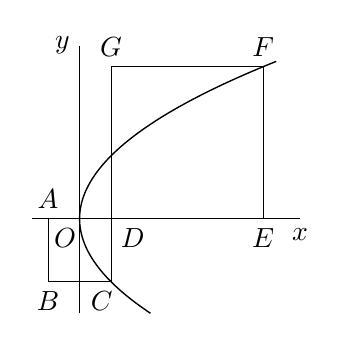
\begin{tikzpicture}[scale=0.4]
      \draw[\myaxisarrow] (-1.5,0) -- (7,0) node[below] {$x$};
      \draw[\myaxisarrow] (0,-3) -- (0,5.5) node[left] {$y$};
      
      \draw[line width=0.5pt,smooth,samples=100,domain=-1.5:2.5,variable=\t] 
        plot({(\t)^2},{2*\t}); % y^2=4x
      
      \draw (0,0) coordinate (O) +(0.2,0) node[anchor=north east] {$O$};
      \draw (-1,0) coordinate (A) node[above] {$A$};
      \draw (-1,-2) coordinate (B) node[below] {$B$};
      \draw (1,-2) coordinate (C) +(-0.3,0) node[below] {$C$};
      \draw (1,0) coordinate (D) node[anchor=north west] {$D$};
      \draw (5.828,0) coordinate (E) node[below] {$E$};
      \draw (5.828,4.828) coordinate (F) node[above] {$F$}; 
        % (3+2\sqrt2,2+2\sqrt2)
      \draw (1,4.828) coordinate (G) node[above] {$G$};
      
      \draw (A)--(B)--(C)--(G)--(F)--(E);      
    \end{tikzpicture}
    \caption{}\label{fig-190629-1500}
    \end{figure}
    
\subsection{课后练习}
\begin{exercise}
    已知抛物线 $C_1\colon x^2 =2py$ ($p>0$) 的焦点 $F$ 在抛物线 $C_2\colon y= \dfrac12 x^2 +1$ 上, 求抛物线 $C_1$ 的准线方程.
\end{exercise}
\beginsolution
    点 $F$ 在 $y$ 轴上, 故 $F(0,1)$, $C_1$ 的准线方程为 $y=-1$.
\endsolution

\begin{exercise}
    已知抛物线 $C\colon x^2 =4y$ 的焦点为 $F$, 点 $P$ 在 $C$ 上且到 $x$ 轴的距离与 $|PF|$ 之比为 $1:3$, 求点 $P$ 到 $x$ 轴的距离.
\end{exercise}
\beginsolution
    准线 $l\colon y=-1$. 设 $P(x_0,y_0)$, 则 $y_0>0$, 且
    \[y_0: |PF|= y_0: (y_0+1)= 1: 3,\]
    所以 $y_0= \dfrac12$, 即为所求距离.
\endsolution

\begin{exercise}
    若抛物线 $C\colon y^2 =2px$ 上一点 $Q(4, q)$ 到其焦点 $F$ 的距离为 $5$, 求 $q$ 的值.
\end{exercise}
\beginsolution
    准线 $l\colon x= -\dfrac{p}2$, 则
    \[|QF|= 4+\frac{p}2= 4,\quad p=2.\]
    将 $Q(4, q)$ 代入 $C\colon y^2 =2px$,
    \[q^2= 2\cdot 4\cdot 8,\quad q= \pm8.\]
\endsolution

\begin{exercise}
    已知抛物线 $C\colon y^2= 4x$ 的焦点为 $F$, 准线 $l$ 与 $x$ 轴的交点为 $A$, 点 $P$ 在 $C$ 上且 $|PA|= \dfrac{\sqrt5}2 |PF|$, 求 $\triangle PFA$ 的面积. 
\end{exercise}
\beginsolution
    $F(1,0)$, $l\colon x=-1$, $A(-1,0)$. 设 $P(x_0,y_0)$.

    方法一: 由 $|PA|= \dfrac{\sqrt5}2 |PF|$ 知,
    \[\sqrt{(x_0+1)^2+ y_0^2}= \frac{\sqrt5}{2}(x_0+1),\]
    将 $y_0^2= 4x_0$ 代入得
    \[x_0^2- 14x_0+ 1= 0,\quad x_0= 7\pm 4\sqrt3.\]
    所以
    \mymarginpar{这里计算开方需要一点配方技巧.}
    \[y_0^2= 4(7\pm 4\sqrt3),\quad y_0= 2(2\pm\sqrt3),\]
    而 $\triangle PFA$ 的面积
    \[S_{\triangle PFA}= \frac12\cdot |AF|\cdot |y_0|
    = 2(2\pm\sqrt3).\]

    方法二: 过点 $P$ 作 $PB\perp l$ 于点 $B$. 由 $|PA|= \dfrac{\sqrt5}2 |PF|$ 设 $|PF|= 2k$, $|PA|= \sqrt5k$, 则
    \[|PB|= |PF|= 2k,\quad |AB|= k.\]
    不妨设 $P(2k-1,k)$, 代入 $C$ 的方程,
    \[k^2= 4(2k-1),\quad k=4\pm 2\sqrt3.\]
    故 $\triangle PFA$ 的面积
    \mymarginpar{用几何法可以简化计算.}
    \[S_{\triangle PFA}= \frac12\cdot |AF|\cdot k
    = 2(2\pm\sqrt3).\]
\endsolution

\begin{exercise}
    如图 \ref{fig-190629-1510} 所示, 抛物线 $C\colon y^2 =2px$ ($p>0$) 的焦点为 $F$, 准线为 $l$, 点 $A(4,y_0)$ ($y_0>0$) 到 $l$ 的距离等于 $5$, 过点 $A$ 作 $AB$ 垂直于 $y$ 轴, 垂足为 $B$, $OB$ 的中点为 $M$.
    
    (1) 求抛物线 $C$ 的方程;
    
    (2) 过点 $M$ 作 $MN\perp FA$, 垂足为 $N$, 求点 $N$ 的坐标.
\end{exercise}
\beginsolution
    (1) $F\Bigl(\dfrac{p}2,0\Bigr)$, $l\colon x=-\dfrac{p}2$, 点 $A$ 到 $l$ 的距离为
    \[4+\frac{p}2= 5,\quad p=2,\]
    则 $C\colon y^2= 4x$.

    (2) 由 (1) 知, $A(4,4)$, $F(1,0)$, 则 $B(0,4)$, $M(0,2)$, 而
    \[AF\colon y= \frac43(x-1),\quad
    MN\colon y= -\frac34 x+2,\]
    联立解得, $N\Bigl(\dfrac85,\dfrac45\Bigr)$.
\endsolution

    \begin{figure}[htb]
    \small
    \centering
    \begin{minipage}[b]{0.45\linewidth}
      \centering
      \begin{tikzpicture}[scale=0.4]
        \draw[\myaxisarrow] (-1.5,0) -- (5.5,0) node[below] {$x$};
        \draw[\myaxisarrow] (0,-3) -- (0,5) node[left] {$y$};
        
        \draw[line width=0.5pt,smooth,samples=100,domain=-1.5:2.2,variable=\t] 
          plot({(\t)^2},{2*\t}); % y^2=4x
        
        \draw (0,0) coordinate (O) node[anchor=north east] {$O$};
        \draw (4,4) coordinate (A) node[above] {$A$};
        \draw (0,4) coordinate (B) node[left] {$B$};
        \draw (1,0) coordinate (F) node[below] {$F$};
        \draw (0,2) coordinate (M) node[left] {$M$};
        \draw ($(A)!(M)!(F)$) coordinate (N) node[right] {$N$};
        
        \draw (B)--(A)--(F) (M)--(N) (-1,4.4)--(-1,-3);
        \draw (-1,-2) node[left] {$l$};
      \end{tikzpicture}
      \caption{}\label{fig-190629-1510}
    \end{minipage}
    \hskip 0.5cm  
    \begin{minipage}[b]{0.45\linewidth}
      \centering
       \begin{tikzpicture}[scale=0.4]
         \draw[\myaxisarrow] (-1.5,0) -- (6,0) node[below] {$x$};
         \draw[\myaxisarrow] (0,-3) -- (0,5) node[left] {$y$};
         
         \draw[line width=0.5pt,smooth,samples=100,domain=-0.5:0.9,variable=\t] 
           plot({6*(\t)^2},{6*\t}); % y^2=6x
         
         \draw (0,0) coordinate (O) node[anchor=north east] {$O$};
         \draw (3.5,4.5826) coordinate (A) node[above] {$A$}; 
           % (7/2,\sqrt{21})
         \draw (0.5,1.732) coordinate (B) +(-0.15,0) node[above] {$B$};
           % (1/2,\sqrt3)
         \draw (1.5,0) coordinate (F) node[below] {$F$};
         \draw (5,0) coordinate (E) node[below] {$E$};
         \draw ($(A)!(C)!(B)$) coordinate (D) +(-0.15,0) node[above] {$D$};
         
         \draw (A)--(B)--(F)--(A) (D)--(E);      
       \end{tikzpicture}
       \caption{}\label{fig-190629-1520}
    \end{minipage}
    \end{figure}
    
\begin{exercise}
    如图 \ref{fig-190629-1520} 所示, 已知抛物线 $C\colon y^2 =6x$ 的焦点为 $F$, 两个动点 $A$ 和 $B$ 在 $C$ 上且满足 $|AF|+|BF|=7$, 线段 $AB$ 的中点为 $D$, $DE\perp AB$ 且与 $x$ 轴交于点 $E$, 求点 $E$ 的坐标.
\end{exercise}
\beginsolution
    $F\Bigl(\dfrac32,0\Bigr)$, 准线 $l\colon x=-\dfrac32$. 设 $A(x_A,y_A)$, $B(x_B,y_B)$, 则
    \[\begin{aligned}
        |AF|+|BF|
        &= \Bigl(x_A+\frac32\Bigr)+ \Bigl(x_B+\frac32\Bigr)\\
        &= x_A+x_B+3= 7,
    \end{aligned}\]
    所以 $x_A+x_B= 4$. 设 $E(x_E,0)$, 则 $|EA|= |EB|$, 则
    \[(x_E-x_A)^2+ y_A^2= (x_E-x_B)^2+ y_B^2,\]
    整理并结合 $y_A^2= 6x_A$ 和 $y_B^2= 6x_B$ 得,
    \mymarginpar{也可以先写出 $DE$ 的方程, 再求其与 $x$ 轴的交点 (令纵坐标为 $0$).}
    \[\begin{aligned}
        2x_E
        &= \frac{x_A^2-x_B^2}{x_A-x_B}+ \frac{y_A^2-y_B^2}{x_A-x_B}\\
        &= x_A+x_B+ \frac{6x_A-6x_B}{x_A-x_B}\\
        &= 4+6= 10,
    \end{aligned}\]
    所以 $x_E= 5$, $E(5,0)$.
\endsolution